\section{Marco de Desarrollo OpenSARA}

openSARA es un marco de desarrollo experimental para aplicaciones PHP orientadas a la web. Se desarrolló con el objetivo de simplificar el desarrollo de openSITEM con una orientación hacia programadores. En ese sentido, está pensado para desarrollo ágil de módulos inéditos y el reciclaje de módulos preexistentes. El código base se distribuye bajo licencia Eclipse Public License o GPL. Los diferentes plugins se distribuyen de conformidad a la licencia definida por sus autores. 

openSARA es un marco de trabajo basado en el patrón Frontera - Control - Entidad. La conexión a bases de datos se abstrae por medio de un componente que implementa el patrón \textit{Abstract Factory}. 

\begin{figure}
 \centering
 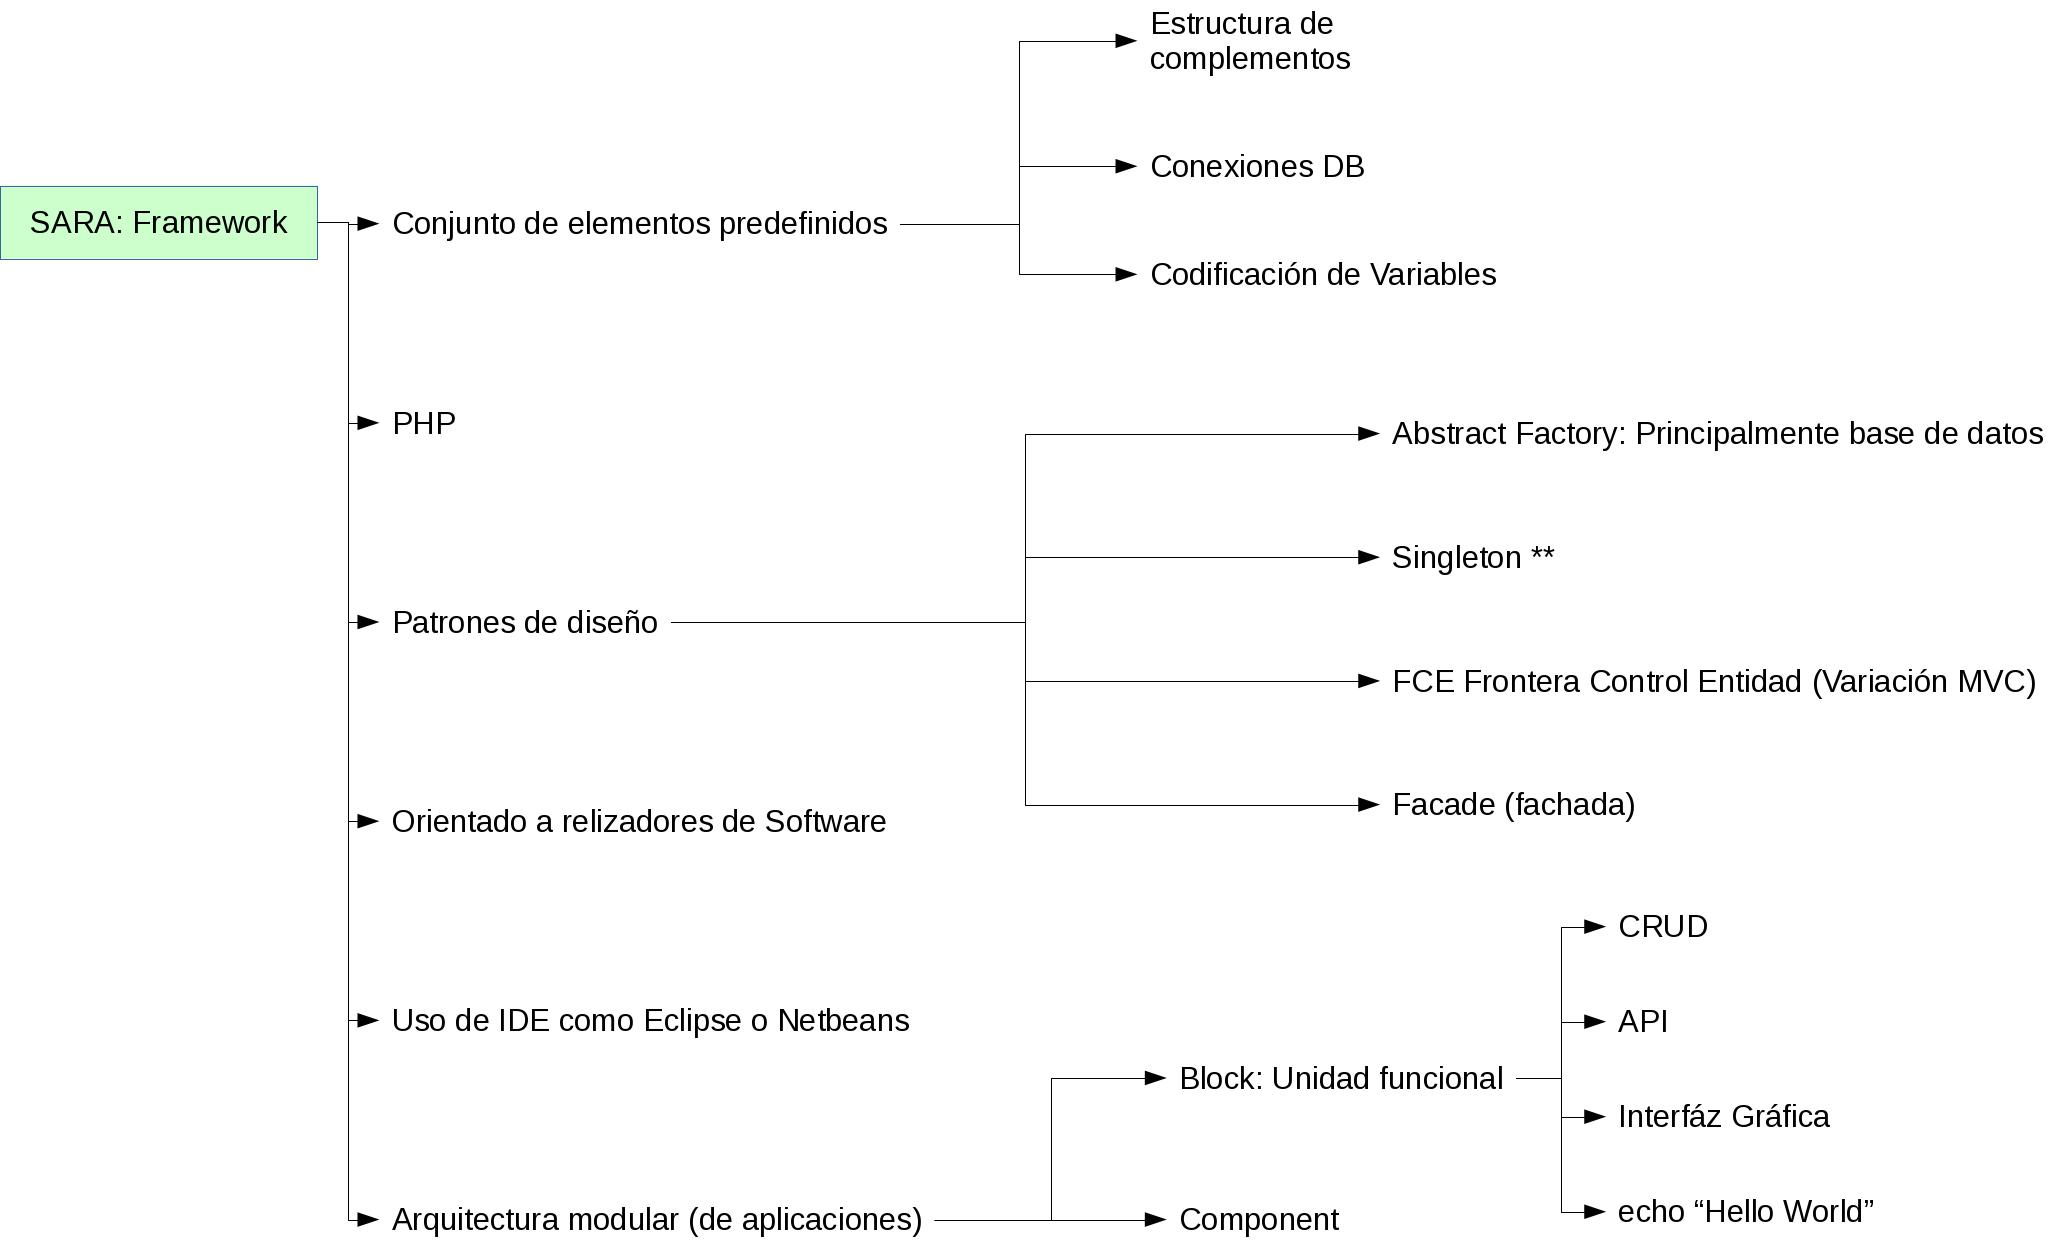
\includegraphics[width=156mm]{openSARA.png}
 \caption{Conceptos principales de OpenSARA}
 \label{aplicaciones_sitem}
\end{figure}


\subsection{Patrón Frontera -Control - Entidad}

Es una variación del patrón Modelo - Vista - Controlador, en donde se hace un mayor énfasis en el bajo acoplamiento. 

\begin{itemize}
 \item Frontera: Objetos que actúan como interfaces del aplicativo con sistemas cliente tales como: usuario humanos, servicios web, aplicaciones heredadas (legacy applications), Interfaces de Programación de Aplicaciones, etc.
 \item Control: Objetos de interoperación entre los objetos frontera y los objetos entidad. Su misión es orquestar la ejecución de la aplicación y la interacción con los sistemas cliente.
 \item Entidades: Objetos que implementan la lógica de negocio. Incluyen aquellos objetos que representan el modelo de datos de las aplicaciones.
\end{itemize}


Los objetos Fontera, Control y Entidad tienen símbolos específicos en el estándar UML.

\subsection{Marco de Trabajo}

\subsubsection{Bloque}
Elemento modular base de openSARA. Puede implementar todo un caso de uso - utilizando patrón FCE, o estar constituido por un simple archivo HTML o PHP. Depende del programador decidir las características del bloque conforme a los requisitos del proyecto. 

OpenSARA recomienda tres modelos de bloques: CRUD completo síncrono, CRUD completo asíncrono (vía AJAX) y servicio web.

\subsubsection{Página}
Punto de interacción con el usuario. Son generadas en tiempo de ejecución con base en la estructura de bloques declarada en base de datos o archivos XML. Una página es creada a partir del código fuente de un conjunto de bloques. Es la interfaz gráfica de la aplicación.

\subsubsection{Clase Nuclear}
Conjunto de clases que gestionan la integración de aplicaciones, se dividen en siete categorías que se encargan de:

\begin{itemize}
 \item Builder: construir las páginas enlazando los diferentes bloques que las constituyen.
 \item Connection: conectar a bases de datos.
 \item Crypto: codificar y decodificar cadenas de petición.
 \item Auth: autenticación, autorización y control de sesiones.
 \item Manager: gestionar el marco de trabajo.
 \item Locale: Internacionalización
 \item General: implementar comportamiento genérico requerido por otras clases nucleares.
\end{itemize}

\subsubsection{Componentes}
Bloque especializado. Un componente se construye con el objetivo de que sea consumido por los bloques cuando se requiere un comportamiento genérico (enviar correos electrónicos, generar notificaciones, gestionar logs, etc). Los componentes definen un contrato a través de las interfaces que declaran.
Complementos

\subsection{Estructura}

\subsubsection{Bloque}
Se ubican dentro de la carpeta blocks y se registran en la base de datos o en archivos XML dependiendo de la configuración del marco de trabajo. Un bloque es una carpeta que debe tener, como mínimo, un archivo llamado bloque.php, el cual se utiliza como punto de entrada (entry point). Aunque esta es la única restricción que impone  openSARA para la estructura, el marco de desarrollo provee dos modelos de bloques enriquecidos que implementan el patrón FCE, el primero de ellos, llamado bloqueModelo1, está compuesto por:


\begin{figure}
 \centering
 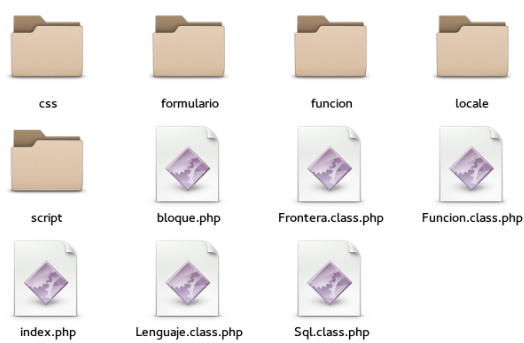
\includegraphics[width=100mm]{carpetaBloque.png}
 \caption{Estructura de un bloque en el sistema de archivos}
 \label{aplicaciones_sitem}
\end{figure}

\begin{itemize}
 \item bloque.php: Clase Bloque que crea los objetos que procesarán las peticiones. Es el elemento de control en el patrón FCE.
 \item Frontera.class.php: Clase Frontera, define la gestión de la interfaz de usuario a partir de los formularios especificados dentro de la carpeta formulario. Implementa el elemento Frontera en el patrón FCE.
 \item Funcion.class.php:  Clase Función, define el procesamiento de los formularios basado en la gestión de objetos creados a partir de las clases de la carpeta funcion. Implementa el elemento Entidad en un patrón FCE.
 \item Lenguaje.class.php: Clase Lenguaje, define las funciones de internacionalización específicas para el bloque, describiendo el procesamiento de los archivos de la carpeta locale.
 \item Sql.class.php: Clase SQL. Define las cadenas SQL que serán utilizadas en el bloque.
 \item Carpeta script: Contiene los archivos js que se utilizarán en el bloque.
 \item Carpeta css: Archivos CSS que definen los estilos que serán aplicados a los elementos del bloque
\end{itemize}